\documentclass{beamer}
\mode<presentation>
{
  \usetheme{Warsaw}
  \setbeamercovered{transparent}
}
\usepackage{tikz}
\usepackage[pdflatex]{graphicx}
\usepackage[utf8]{inputenc}
\usepackage[francais]{babel}
\usepackage{pstricks-add}
\title[Réseaux Sociaux]
{Les Réseaux Sociaux}
\subtitle
{Quelle utilité?}
\author[Verdier, Lameira]{Frédéric~Verdier\and Yannick~Lameira}
\institute[Université Montpellier 2]
{Licence 3 Informatique}
\date[2012] 
{Conduite de projet}
\begin{document}
\begin{frame}
  \titlepage
\end{frame}
\begin{frame}{Plan}
  \tableofcontents
\end{frame}
\section{Qu'est-ce qu'un réseau social?}
\subsection{Définition}
\begin{frame}{Définition}
  \begin{itemize}
  \item
    Un réseau social est un ensemble d'identités sociales, telles que des individus ou encore des organisations, reliées entre elles par des liens créés lors d'interactions sociales.
  \item
    Certains « réseaux sociaux » sur Internet regroupent des amis de la vie réelle. D'autres aident à se créer un cercle d'amis, à trouver des partenaires commerciaux, un emploi ou autres. Il s'agit de services de réseautage social, comme Facebook, Twitter, Identi.ca, MySpace, Viadeo, Instagram ou LinkedIn.
  \end{itemize}
\end{frame}
\subsection{Historique}
\begin{frame}{Historique}{Quelques dates importantes}
	\begin{itemize}
		\item 1997 : naissance de l'un des premiers réseaux sociaux : Sixdegrees.
		\item 2001 : lancement du réseau social professionnel : Ryze.
		\item 2003 : lancement de Friendster (février) Linkedin (mai), Myspace (août) et Xing (novembre). Début du web 2.0
		\item 2004 : la concurrence s'accentue avec Orkut (janvier, propriété de Google), Facebook (février) et Viaduc (futur Viadeo).
		\item 2005 : création de Youtube.
		\item 2006 : création de la plateforme de micro-blogging Twitter.
		\item 2011 : entrées en bourse de Linkedin et Renren, présent en Chine (mai). Lancement de Google +.
		\item 2012 : entrée en bourse de Facebook.
	\end{itemize}
\end{frame}

\section{Différents utilisateurs pour différentes utilisations}

\subsection{Les réseaux tout public}
\begin{frame}{Les réseaux tout public}
	Ce type de réseau social vise une population très variée. \\
	Ce sont les réseaux sociaux comptant le plus de membre et plus généralement le plus de visites.\\
	Ces réseaux peuvent diffuser les informations soit sur un unique support soit sur plusieurs...
\end{frame}

\begin{frame}{Les réseaux tout public}{Partage d'informations sur divers supports}
	Les grands représentants de ce genre de réseaux sont \textit{Facebook} et \textit{Twitter}.
	\\\textbf{Utilités : }
	\begin{itemize}[<+-| alert@+>]
		\item Chaque utilisateur connecté peut accéder aux informations publiées par les autres utilisateurs selon ses droits d'accès (ami ou non...)
		\item Permet de partager des informations sur des supports variés (images, vidéos, textes) et de les commenter.
		\item Permet de rejoindre des groupes de personnes pour discuter ou afficher une opinion particulière.
		\item Permet de rencontrer d'autres utilisateurs via ses propres amis, groupes...
		\item Fournis des applications variées (sur Facebook des jeux, calendrier, messagerie instantanée...).
	\end{itemize}
\end{frame}

\begin{frame}{Les réseaux tout public}{Partage d'informations à support restreint}
	Ce genre de réseaux se focalisent sur un support unique d'informations pour créer des liens entre différents utilisateurs.\\
	On retrouve \textit{Youtube} (partage de vidéos) et \textit{Picassa} (partage de photos).\\
	\textbf{Utilités : }
	\begin{itemize}[<+-| alert@+>]
		\item Permet de partager ses informations à tout autre utilisateur dans un format donné.
		\item Permet à tout utilisateur de regarder ce que les membres du réseau postent.
		\item Permet de commenter et critiquer la pertinence de l'information.
	\end{itemize}
\end{frame}

\definecolor{myblue}{HTML}{92dcec}
\begin{tikzpicture}
    \foreach \start/\end/\middle/\percent/\anchor/\name/\smeter in {
      0/72/36/20/above/13-17/,
      72/90/81/5/above/55-64/,
      90/118/104/8/left/45-54/,
      118/172/135/15/above/35-44/,
      172/266/219/26/left/18-25/,
      266/360/313/26/right/26-34/}
  {
    \draw[fill=myblue, thick] (0,0) -- (\end:3cm) arc (\end:\start:3cm)
      node at (\middle:1.8cm) {\percent \%};
    \draw (\middle:3cm) -- (\middle:3.5cm) node[\anchor] {\name \ \smeter ans};
  };
\end{tikzpicture}
\subsection{Les réseaux à public ciblé}
\begin{frame}{Les réseaux à public ciblé}{Partage d'informations sur un thème particulier}
	Ce sont des réseaux ciblant une catégorie de personnes ou entités.\\
	Ces réseaux sont moins fréquentés que les réseaux tout public mais propose généralement des services plus poussés dans leur domaine.\\
	Ce sont des réseaux qui ont souvent un système de souscription au moins partiel à des comptes payants pour avoir tous les avantages du réseau.\\
	\textbf{Utilités : }
	\begin{itemize}
		\item Permet de partager des informations relatives au thème du réseau (C.V. pour LinkedIn, description de la personnalité dans Meetic, ...) .
		\item Propose des services et applications variés adaptés aux besoins de l'utilisateur (affichage des actualités des entreprises en fonction du métier recherché dans LinkedIn, ...).
	\end{itemize}
\end{frame}
\section{Les intérêts commerciaux}
\subsection{Les stratégies majeures d'expansion}
\begin{frame}{Les intérêts commerciaux}{Les stratégies majeures d'expansion}
Les réseaux sociaux ont pour objectif d'attirer toujours plus de membres. Pour cela il existe deux stratégies majeures : 
	\begin{itemize}
		\item Les réseaux tout public fournissent des services divers pouvant être apprécié par la majeure partie des utilisateurs d'Internet (Facebook, Twitter, Youtube, ...). Ce sont généralement des serveurs qui ont un système de souscription gratuite. Ils louent leur espace à des agences publicitaires, leur nombre de membres faisant leur crédibilité.
		\item Les réseaux ciblés cherchent une catégorie particulière de personnes, de besoins afin d'y répondre plus efficacement. Leur droit de souscription est souvent payant vu que leur nombre de membres est plus restreint.
	\end{itemize}
\end{frame}
\subsection{Quelques chiffres}
\begin{frame}{Les intérêts commerciaux}{Quelques chiffres}
\begin{itemize}
	\item 75\% des utilisateurs d'Internet dans le monde utilisent au moins un réseau social.
\end{itemize}
	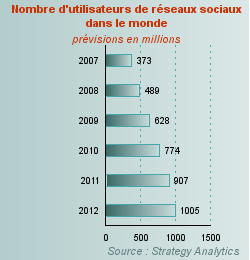
\includegraphics[width=10cm, height=5cm]{graphe1.png}
\end{frame}
\begin{frame}{Les intérêts commerciaux}{Quelques chiffres}
	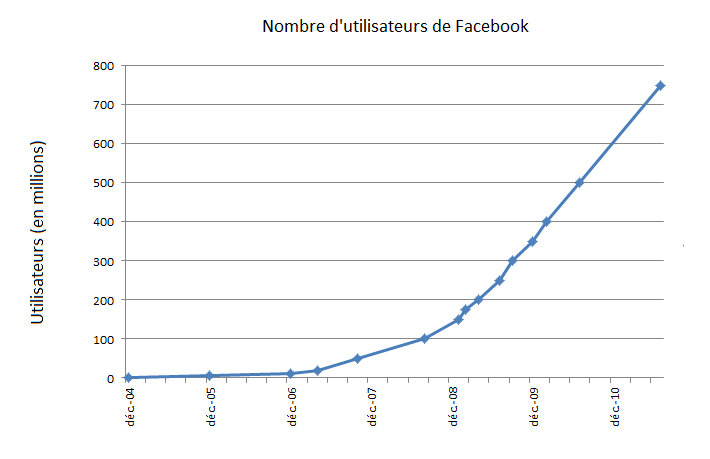
\includegraphics[scale=0.5]{Facebook_users_fr.png}
\end{frame}
\section{Les dangers de l'utilisation des réseaux sociaux}
\subsection{Quelques scandales}
\begin{frame}{Les dangers de l'utilisation des réseaux sociaux}{Quelques scandales}
	\begin{itemize}
		\item 26 mais 2010 : Inj3ctor capte des données bancaires via les données personnelles d'utilisateurs de Facebook.
		\item 21 mai 2010 : Envois de données personnelles sans le consentement des utilisateurs à des annonceurs comme Google Double Click et Yahoo's Right Media par Facebook.
		\item 6 juin 2012 : Vol de données personnelles et confidentielles dans les bases de données de LinkedIn.
		\item Des salariés licenciés après avoir publié des critiques sur leur entreprise sur Facebook.
		\item Des messages privés affichés en "clair" sur Facebook.
	\end{itemize}
\end{frame}
\subsection{Les litiges entre vie privée et réseaux sociaux}
\begin{frame}{Les dangers de l'utilisation des réseaux sociaux}{Les litiges entre vie privée et réseaux sociaux}
	Les réseaux sociaux en général conservent toutes les informations, personnelles ou non, que les utilisateurs diffusent. \\
	Ils peuvent les utiliser pour faire de la publicité ciblée sur les centres d'intérêts, la personnalité ou le statut social de la personne\\
	Les informations personnelles peuvent être vendues à des annonceurs ou d'autres organismes publicitaires.\\
	Les données publiées sur les réseaux sociaux sont vulnérables aux attaques, aux détournements...\\
\end{frame}


\section*{Conclusion}

\begin{frame}{Conclusion}
  \begin{itemize}
  \item Les réseaux sociaux sont utiles car ils \alert{permettent de connecter toute sorte d'entités afin d'échanger des idées, de créer des liens ou d'évaluer la qualité d'une information} par l'intelligence collective. 
  \item Avec un nombre important d'utilisateurs, \alert{le marché des réseaux sociaux autours de la publicité et des souscriptions payantes est devenu très disputé.} Ce monde en perpétuelle mutation a vu en quelques années l'émergence de Facebook ou LinkedIn dont le chiffre d'affaire est colossal.
  \item Cependant, \alert{les abus et autres trafics d'informations personnelles des utilisateurs sont des dangers} nous poussant à douter de l'apport bénéfique des réseaux sociaux.
  \end{itemize}
\end{frame}
\appendix
\section<presentation>*{\appendixname}
\subsection<presentation>*{Bibliographie}
\begin{frame}[allowframebreaks]
  \frametitle<presentation>{Bibliographie}  
  \begin{thebibliography}{10} 
  \beamertemplatebookbibitems
  \bibitem{wiki}  http://www.wikipedia.org
  \bibitem{infonet} http://www.infos-du-net.com
  \bibitem{droit} http://loi.blogs.liberation.fr
  \bibitem{linkedin} http://www.welovebuzz.com
  \bibitem{bug} http://www.20min.ch
  \end{thebibliography}
\end{frame}

\end{document}